\section{Design}
\subsection{Overview}
\begin{comment}
\begin{figure}[t!]
	\centering
	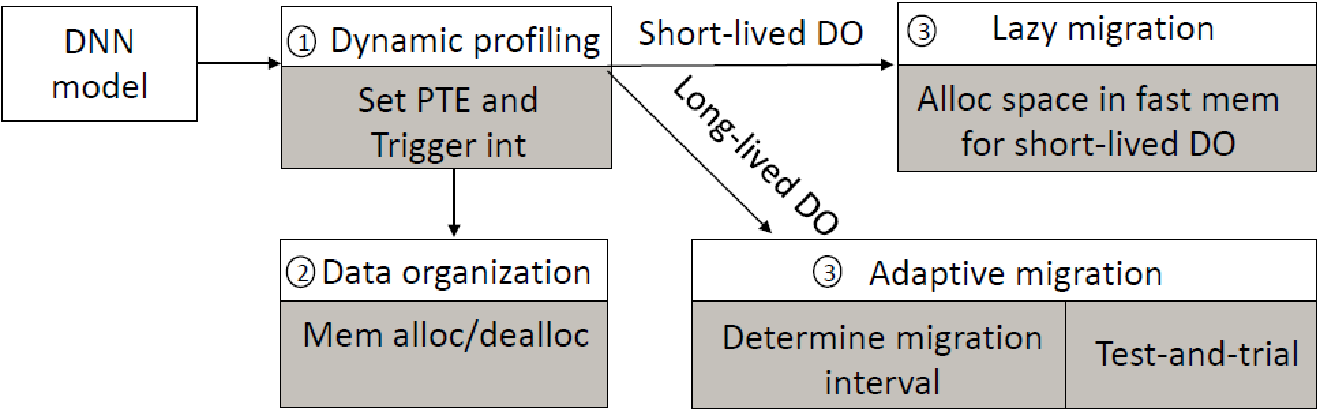
\includegraphics[height=0.11\textheight]{./figures/overview-2.pdf}
	\vspace{-5pt}
	\caption{Overview of \name. ``DO'' stands for ``data object''.  The white and shadow boxes represent functionality and mechanisms, respectively.} 
	\vspace{-15pt}
	\centering
	\label{fig:overview} 
\end{figure}
\end{comment}

%\name consists  of multiple components, shown in Figure~\ref{fig:overview}. The dynamic profiling component 
\textcolor{check}{\name uses dynamic profiling to }collect memory access information at the data object level, and decides the lifetime of data objects based on customized memory allocation and limited user annotation (Section~\ref{sec:dyn_profiling_data_org}). The dynamic profiling uses only one training step to collect the information. After that, \name re-organizes memory allocation for short-lived data objects to facilitate data management and avoid page-level false sharing.

Driven by the profiling results, \name treats short-lived and long-lived data objects separately (Section~\ref{sec:short-lived}). Short-lived data objects are allocated in contiguous memory space in fast memory, and are not involved in data movement between fast and slow memories. This method avoids inefficient data movement due to short liveness. 

To handle long-lived data objects, \name uses an adaptive migration algorithm  (Section~\ref{sec:adaptive_dm}). The algorithm partitions each training step into migration intervals, based on the DNN model topology. In a migration interval, \name migrates data objects needed for the next interval, overlapping application execution with data migration. During data migration, \name must determine an appropriate migration interval, such that the data objects can be timely migrated from slow to fast memory before they are needed by DNN training. We formulate the problem and determine the optimal migration interval. We also use a test-and-trial algorithm to determine if the migration cannot happen timely, whether continuing migration or not can lead to better performance. 


%In general, \name uses the following domain knowledge to enable high performance of DNN training. 
%\begin{itemize}
%    \item Repetitiveness of DNN training for profiling and predicting memory access patterns;
%    \item The liveness of data objects (tensors) within and across layers to decide data migration;
%    \item The DNN model topology (i.e., layers) and \textcolor{dong2}{its depth} to decide the optimal migration interval and trigger data migration.
%\end{itemize}





\subsection{Dynamic Profiling and Data Reorganization}
\label{sec:dyn_profiling_data_org}

%\textbf{Dynamic profiling.} 
%\name integrates the profiling framework in Section~\ref{sec:profiling_framework} into the TensorFlow runtime system. We favor dynamic profiling instead of static one, although the static dataflow graph can be known before the training starts, because thread-level parallelism within an operation and across operations cannot be captured by static profiling. Such parallelism has significant impacts on data locality.  %Our profiling method uses \textcolor{red}{xxx\%} of total training time, which is a rather small overhead.


%textcolor{green}{We adopt the profiling flamework to get combined data access information in page-level and application-level for online profiling. The online profiling method is critical for the data migration on machine learning flamework since the data access are various between different parallelism strategy. Our online profiling method brings 4\% to 8\% runtime overhead. Leveraging the remarkable predictability of DNN model, Sentinel only needs to profile one training step(i.e, one mini-batch) to get data access information. Considering of DNN models usually needs tens of thousands of training steps to converge, the online profiling overhead is lightweight.}

%\textcolor{green}{All tensor allocation happens in slow memory during the profiling such that ensures there are enough space for tensor allocation. During the profiling, we maintain information of each data which used in one training step as data lifetime and size, and the access time in each operation.}\textcolor{blue}{Todo: why os level profiling with allocate each tensor pre-page.}

\name integrates the profiling framework in Section~\ref{sec:profiling_framework} into the TensorFlow runtime. \textcolor{check}{\name skips the first 10 training steps which are usually used by the machine learning framework to detect hardware configuration, and uses the 11th training step for profiling.}

%\textcolor{jie}{We use the term "tensor" instead of "data object" for the following discussion, will that make inconsistency?}

\textcolor{check}{Based on the profiling results, \name uses a customized memory allocation policy in the remaining training steps, described as follows. (1) For those short-lived data objects alive in the same layer, they are allocated into the same pages, because of their same live time and a similar number of memory accesses. (2) For those long-lived data objects that reside in the exact same layers, we use the following algorithm to determine their memory co-allocation. We first sort them in terms of the number of memory accesses in descending order, and then allocate them in contiguous memory pages, following the descending order. As a result, data objects with %a similar number of memory accesses 
\textcolor{check}{the similar memory access pattern} %(i.e., be accessed in same layers) 
can be allocated into the same memory pages. (3) For those long-lived data objects that do not reside in the same layers, they never share any memory page. (4) Long- and short-lived data objects never share any memory page. 
}

%\textcolor{jie}{Based on the profiling results, \name uses a customized memory allocation for the remaining training steps. In particular, data objects that have the similar memory access pattern (including number of accesses and memory allocation and deallocation times) are allocated into the same page, in order to avoid page-level false sharing and reduce TLB misses. This is implemented by associating a bit string with each data object. The bit string indicates which layer this data object is accessed. Data objects that have the same bit string are grouped. Data objects falling into the same group are sorted in terms of number of memory accesses. }

\textcolor{check}{
The above data reorganization in the \textit{profiling and regular training steps} happens to long- and short-lived data objects allocated in the middle of the training process.  Those data objects are allocated and freed in each training step, allowing us to reorganize them across training steps without impacting program correctness. A few long-lived data objects (e.g., weights and input samples) that are allocated before the training process cannot be reorganized in the middle of training processing, because that will change memory addresses of those data objects and cause wild pointers. Those data objects never share pages during memory allocation, in order to avoid page-level false sharing and unnecessary data migration. 
}


%\textcolor{jie}{In the implementation, \name preallocates fast memory as the size specified by the user. \name manages the fast memory for short-lived and long-lived data objects separately. \name reserves a continues fast memory space for short-lived data objects. Since those data objects are frequently allocated and freed, using the memory pool can avoid repeatedly returning memory to the system, mitigating unnecessary overhead. For short-lived data objects, \name allocate them with the best fit strategy in the reserved space to make the best use of reserved fast memory space. The remaining preallocated fast memory space is for long-lived data objects. The long-lived data objects in a group are allocated and packed into the same set of pages, following the increasing order. Long-lived data objects in different groups do not share memory page. \name migrates pages base on the bit string of data objects allocated on this page.}

\begin{comment}
Based on the profiling results, \name uses a customized memory allocation for the remaining training steps. In particular, short-lived data objects that have the similar memory access pattern (including number of accesses and memory allocation and deallocation times) are allocated into the same page, in order to avoid page-level false sharing and reduce TLB misses. This is implemented by associating a bit string with each data object. The bit string indicates which layer this data object is accessed. Data objects that have the same bit string are grouped. Data objects falling into the same group are sorted in terms of number of memory accesses. 
The data objects in a group are allocated and packed into the same set of pages, following the increasing order.

%%It would be better to elaborate a bit more on your algorithm of reorganizing the objects/page mapping.  Do you regroup short-lived tensors as well long-lived tensors? Do you maintain a queue internally to track the object allocation requests? Is it a ranking + greedy algorithm, does it consider padding?


%\textcolor{green}{\name reorganize the location for short-lived and long-lived data objects. Specifically, \name maintains a bit string to indicate whether data object be accessed in each DNN model layer. \name groups tensors with identical bit string together for allocation. \name allocates data objects in the same group in the same set of pages. }

Furthermore, \name preallocates a memory pool to meet the memory allocation requests for short-lived data objects. Since those data objects are frequently allocated and freed, using the memory pool can avoid repeatedly returning memory to the system, mitigating unnecessary overhead. 
\end{comment}

%\textcolor{jie}{Data objects will similar characteristics(e.g., allocation time, access layers) will be allocated in same memory pages to avoid TLB miss. Short-lived data objects groups together based on their allocation layer. To save limited fast memory space, \name allocates as much short-lived data objects as possible into same memory page. }


%\textcolor{dong}{Memory pre-allocation.} \textcolor{green}{\name allocator pre-allocates heterogeneous memory for tensors for two reasons. Firstly, the default allocator in TensorFlow frequently allocates/deallocates large amount of tensors, which causes unnecessary runtime overhead. \name allocator holds on to released memory rather than releasing to OS directly for better performance. Secondly, the default allocator in TensorFlow allocates tensors without considering tensor access pattern. Allocator in \name allocates tensors with similar access pattern(i,e., tensors with similar access frequency, allocation and deallocation time) according to profiling result, which can reduce unnecessary page migrations and TLB miss.}





%\textcolor{dong}{Data reorganization.} \textcolor{green}{For tensors allocated during the profiling, \name reorganizes them according to profiling result. As Figure~ shows, most of tensors' lifetime is less than one training step. The runtime overhead for reorganizing tensors is ignorable.}
\vspace{-3pt}
\subsection{Handling Short-Lived Data Objects}
\label{sec:short-lived}
%\textcolor{red}{Paragraph: define short-live tensors. }
%\textcolor{green}{\name considers tensor whose lifetime is shorter than one layer.}
%%We define short-lived data objects as those whose lifetime is within one layer. Short-lived data objects are allocated and freed within one layer. %Driven by our profiling results, we treat short-lived and long-lived data objects differently. This section discusses how to handle short-lived data objects, and the next section (Section~\ref{sec:adaptive_dm}) discusses how to handle long-lived data objects. 
During DNN training, an individual short-lived data object is not accessed many times (e.g., less than 10 times in ResNet) in main memory, compared to many long-lived data objects. Hence, the data placement of a specific short-lived data object has an ignorable impact on the performance of DNN training. However, as our profiling results show that there are a large amount of short-lived data objects throughout the whole training process, and they share the same memory access characteristics (i.e., short-liveness, small size, and a small number of accesses in main memory). We must use a general policy to manage them.   

%\textcolor{red}{Paragraph: describe our algorithm that reserves a space in fast memory to handle small data objects}
We use the following algorithm to manage short-lived data objects. We allocate a continuous memory space in fast memory for short-lived data objects. Data objects in this space are never considered for migration. This space is reused for short-lived data objects, as they are allocated and freed 
throughout the training process. The space is %allocated 
\textcolor{dong2}{reserved} at the beginning of each migration interval to accommodate short-lived data objects in the interval. Doing this, \name guarantees that there is always memory space for short-lived data objects (i.e., no competition from long-lived data objects), because the placement of short-lived data objects is critical for performance. 
%dynamically expanded, when there is no free space to accommodate the allocation requests;  
Within a migration interval, space can be dynamically shrunk to free space for long-lived data objects, when a memory page in the space %is freed. 
is no longer needed by short-lived data objects.
%We collect short-lived data objects in this memory space, such that those short-lived data objects allocated and accessed at the similar time can be placed into the same page to avoid page-level false sharing. 


%\textcolor{red}{Paragraph: the reason why we never move short-lived data objects out of fast memory. Mention that the existing algorithm can inappropriately handle short-lived data objects.}
The above method addresses the limitation of the existing methods that use a caching algorithm~\cite{Ramos:ics11, RAMinate:socc16, 5260554, Yan:ASPLOS19, heteros:isca17} or count the number of memory accesses within a time window~\cite{Thermostat:asplos17, unimem:sc17}  \textcolor{check}{to decide data placement}. Those methods move short-lived data objects to slow memory, even though they are not accessed any more. This results in two problems: (1) Unnecessary data movement causes performance loss and wastes memory bandwidth; (2) Short-lived data objects unnecessarily stay longer in fast memory, wasting valuable space in fast memory. The above problems are caused by the fact that making the decision on the movement of short-lived data objects takes some time, due to the necessity of collecting memory access information to run the caching algorithm. Also, counting the number of memory accesses for individual data objects can be inaccurate, because they can share memory pages and the number of memory accesses to each data objects is small. \textcolor{check}{Using our method based on the DNN topology, we do not have the above problems.} 


%\textcolor{red}{Paragraph: what if there is no enough space to hold short-lived data objects? This case will never happen.}
In our design, fast memory is always large enough to host short-lived data objects. If not, short-lived data objects will be frequently moved between fast and slow memories. This data movement is highly inefficient in terms of both performance and energy efficiency. %, especially for data objects with a short lifetime. 
Hence, we assume that the fast memory size is at least larger than the peak memory consumption of those short-lived data objects (discussed in Section~\ref{sec:discussion}). 
%We have a discussion on the fast memory size in Section~\ref{sec:discussion}.  

Since short-lived data objects are frequently allocated and freed and we reuse the same memory space to host them, the size of peak memory space for short-lived data objects is small, and typically bounded by a few GB
\textcolor{check}{, making it feasible to host short-lived objects in fast memory without consuming too much space}. 

\vspace{-7pt}
%\subsection{Adaptive Data Migration}
\subsection{\textcolor{check}{Adaptive Layer-based Migration}}
\label{sec:adaptive_dm}


%\textcolor{dong}{paragraph: basic idea about the data migration and migration interval. Add a figure here?}
%%%We migrate data for those long-lived data objects, 
We migrate long-lived data objects 
\textcolor{check}{because they are used sparsely and periodically}. %and short-lived tensors (if the space of fast memory is not enough to accommodate the upcoming data migration). 
%%%The data migration is controlled by the \textit{migration interval}. The migration interval determines how frequently we migrate data between fast and slow memories. A training step is partitioned into many equal-sized
The data migration is controlled by the \textit{migration interval} \textcolor{check}{which is a system parameter that} determines how frequently we migrate data between fast and slow memories. %%%A training step is partitioned into many equal-sized migration intervals. Figure~\ref{fig:migration_interval} generally depicts data migration.
\textcolor{check}{In particular, we partition a training step (one forward step plus one backward step) into equal-sized intervals, shown in Figure 5.}

Data migration from slow to fast memory is triggered at the beginning of each interval, aiming to prefetching data objects needed by the next interval into fast memory before the next interval starts. The data migration happens in the middle of each interval, in order to overlap data migration with DNN training computation as much as possible, such that the overhead of data migration is removed from the critical path. 

Data migration from fast to slow memory is triggered and happens in the middle of the interval, when the long-lived data object is \textcolor{check}{no longer accessed by any operation in the interval}. Such data migration is used to save the space of fast memory as much as possible, in order to accommodate upcoming data migration. \textcolor{check}{We can know if a long-lived data object will be used by any operation in an interval by using the dynamic profiling results.}
%%\textcolor{red}{%%%We keep a access counter for each long-lived data objects and initialize it with the total access time of this long-lived data objects in current migration interval. 
%%By bookkeeping the long-lived data objects access time and comparing it with profiling result, we can identify whether the long-lived data object will be accessed in current migration interval.}

%and save space for short-lived data objects.
%\textcolor{green}{For each migration interval, \name migrates data into fast memory which will be used in next migration interval execution. Using migration interval ensures \name migrate data for future usage.}

\begin{comment}
\begin{figure*}[htb!]
	\centering
	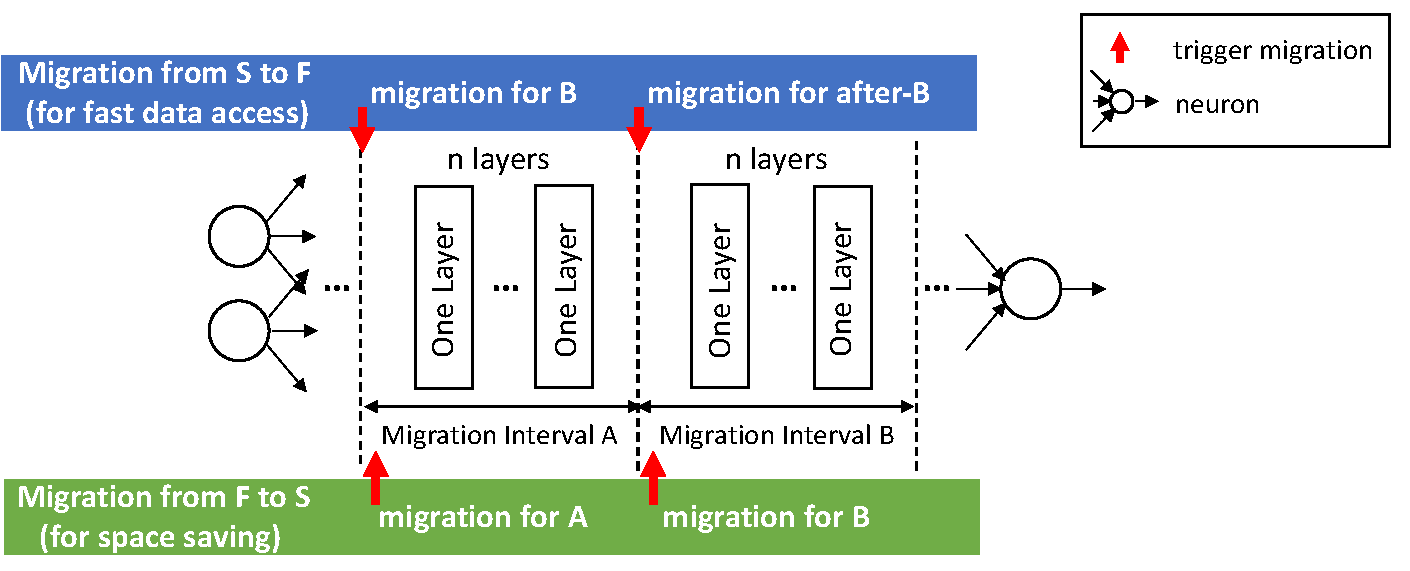
\includegraphics[width=1.0\linewidth, height=0.2\textheight]{./figures/migration_interval.pdf}
	\vspace{-20pt}
	\caption{Data migration based on the migration interval. ``S'' and ``F'' stand for slow and fast memories respectively.} 
	\centering
	\label{fig:migration_interval} 
	\vspace{-5pt}
\end{figure*}
\end{comment}

\begin{figure}
\centering
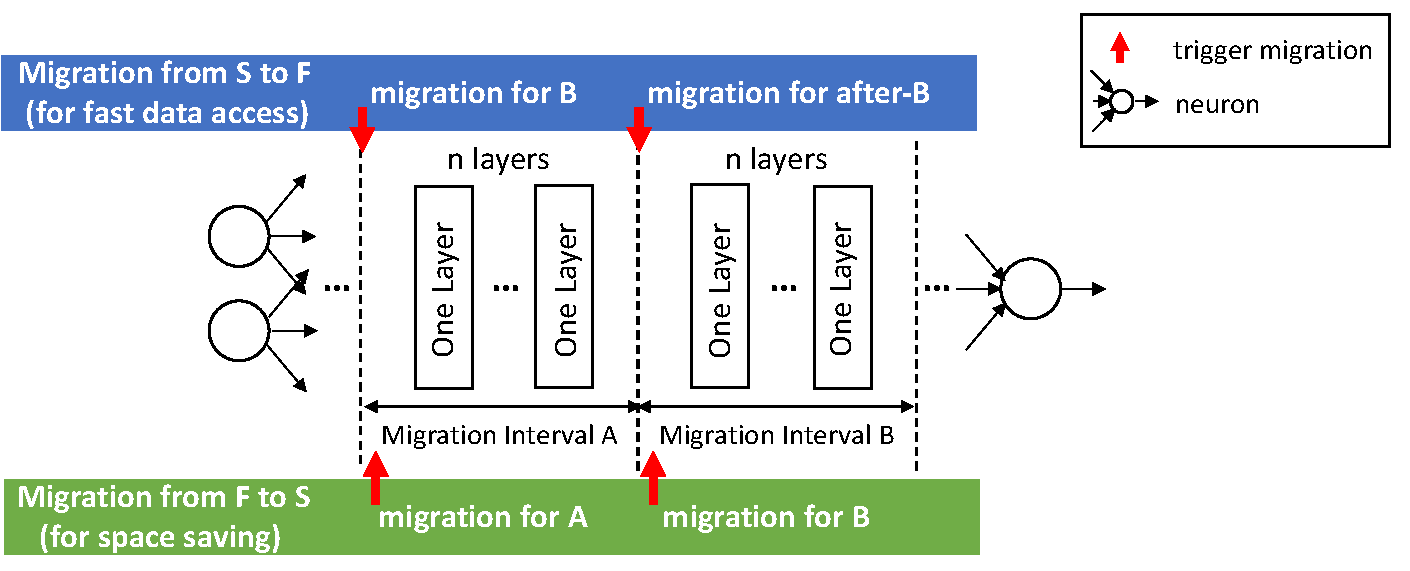
\includegraphics[width=0.48\textwidth]{figures/migration_interval.pdf}
\vspace{-20pt}
\caption{
\textcolor{check}{
Data migration based on the migration interval.  
\textcolor{check}{``S'' and ``F'' stand for slow and fast memories respectively.}}
%\textcolor{dong}{At the beginning of a migration interval, \name triggers bidirectional migration between slow and fast memories. %but for different data objects. ``S'', ``F'' and ``MI'' stand for slow and fast memories, and migration interval respectively.} 
}
	\centering
	\vspace{-15pt}
	\label{fig:migration_interval} 
\end{figure}

%\textcolor{red}{paragraph: the migration interval is defined in terms of layers. why?}
We define the migration interval in terms of layers in DNN, not in terms of execution time, because of the following three reasons. First, the layer-based migration interval naturally guarantees the completion of operations at the end of the interval, because no operation runs across layers. 
%%%\textcolor{jie}{because our profiling results show that no operation runs across layers.}
The time-based migration interval cannot guarantee that, which brings inevitable synchronization between application execution and data migration, causing performance loss. Using the DNN domain knowledge (i.e., the layers), we avoid the above problem. Second, each layer is associated with a computation phase that shows a memory access pattern \textcolor{check}{(e.g., which data objects are  accessed and their lifetime)}. 
%how intensively data object access happens)}. 
The layer-based migration interval allows us to easily leverage the memory access patterns collected at the profiling phase to guide data migration. Third, the time-based migration imposes challenges on deciding which operations are in which migration interval, because  \textcolor{check}{operation-level parallelism  (including inter-op and intra-op)} \textcolor{check}{makes it difficult to predict the execution time of each operation}.

%\textcolor{red}{paragraph: the challenge of determining the migration interval. Large vs. small interval}

\begin{figure}
	\vspace{-5pt}
	\centering
	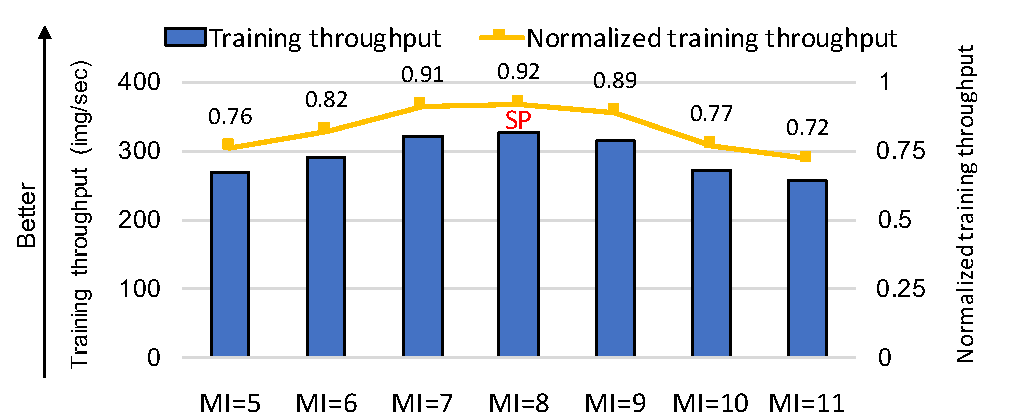
\includegraphics[width=0.48\textwidth]{figures/diff_mi.pdf}
	\vspace{-20pt}
\caption{Performance (training throughput) variance as we change the migration interval (MI). ``SP'' stands for sweet spot (the optimal migration interval).}%\textcolor{green}{Todo}}
\vspace{-10pt}
	\label{fig:optimal_migration_interval}
\end{figure} 


\textbf{Determining an appropriate migration interval} is challenging. If the migration interval is either too large or too small, we cannot achieve the best performance. %\textcolor{red}{paragraph: show the sweet spot of migration interval with figures} 
%To determine the existence of an optimal migration interval, we use different migration intervals and then measure the performance. 
Figure~\ref{fig:optimal_migration_interval} shows the performance when we use different migration intervals for training ResNet\_v1-32 with 1GB fast memory. The figure reveals that the performance is very sensitive to the migration interval. There is 21\% performance variance when we change it from 5 to 11. When the migration interval is 8, we achieve the best performance. Hence, determining an appropriate migration interval is critical for performance.



We analyze the trade-off between large and small migration intervals as follows. If the migration interval is large, then the data to migrate for this interval is large. The migration interval cannot be too large. Otherwise the data to migrate can be larger than the available space in fast memory. This constraint on the migration interval is the \textit{space constraint}, formulated in Equation~\ref{eq:space_constraint}.

If the migration interval is small, then the available execution time to overlap data migration with application execution is short. The migration interval cannot be too short. Otherwise the data to migrate cannot be timely migrated from slow to fast memory before the next migration internal starts. This constraint on the migration interval is the \textit{time constraint}, formulated in Equation~\ref{eq:time_constraint}.

In Equations~\ref{eq:space_constraint} and~\ref{eq:time_constraint} , $RS$ is the fast memory space for short-lived data objects, $S$ is the fast memory size, and $MI$ stands for the migration interval. $RS$ is a function of the migration interval (different migration intervals have different $RS$). In Equation~\ref{eq:space_constraint}, $Data$ is the size of data for migration in a migration interval; In Equation~\ref{eq:time_constraint}, $BW$ is the migration bandwidth from slow to fast memory, and $T$ is the DNN training time in a migration interval. $Data$ and $T$ are functions
% $T$ is a function 
of the migration interval (different migration intervals have different $Data$ and $T$).  

%In both cases, we increase the risk of unfinished data migration before the next migration internal happens. 
%The two constraints establish the upper and lower bounds on the migration interval. There is an optimal migration interval, with which we can maximize the overlap between data migration and application execution and hence minimizes data migration cost.
\vspace{-10pt}
\begin{equation}
%\vspace{-15pt}
\label{eq:space_constraint}
   \text{Space constraint:} \quad Data(MI) < S - RS(MI)  
   %\vspace{-10pt}
\end{equation}
\vspace{-10pt}
\begin{equation}
\label{eq:time_constraint}
   \text{Time constraint:} \quad T(MI) > (S - RS(MI))/BW 
%\vspace{-5pt}
\end{equation}

$RS$ is relatively stable, according to our profiling results. There is a small variance as we change $MI$. Hence $S - RS(MI)$ is near constant. $Data(MI)$ and $T(MI)$ are monotonically increasing functions of $MI$ (i.e., a larger $MI$ indicates larger $Data$ and $T$, and vice versa). Hence, the two equations establish the upper and lower bounds on the migration interval. 

The two equations, although revealing the inherent trade-off between small and large migration intervals, cannot reveal the optimal one, because they do not capture the data movement from fast to slow memory. Such data movement increases the available fast memory space. Because of such data movement, those migration intervals that meet the two constraints can perform differently. 

We use the following method to \textcolor{dong2}{heuristically }determine the optimal migration interval at runtime. After collecting the profiling results, we use Equations~\ref{eq:space_constraint} and~\ref{eq:time_constraint} to prune the search space of the migration interval and choose those that meet the constraints. Then we use a few more training steps, each of which employs a migration interval. We measure their performance, and choose the optimal migration interval that leads to the best performance. %\textcolor{jie}{Below we provide the details of the algorithm. }


%\textcolor{red}{paragraph: discuss the three possible cases at the end of the migration interval.}
\textbf{We encounter three possible data migration cases} at the end of a migration interval. We discuss them as follows. Assume that we have two intervals, $A$ and $B$, and $B$ is right after $A$. \name migrates data at the beginning of $A$ for $B$. At the end of $A$, we have three cases. %The three cases can happen, even if we use the optimal migration interval.
\begin{itemize}[leftmargin=*]
    \item Case 1: All data migration has been finished;
    \item Case 2: Data migration cannot be finished, because fast memory cannot offer enough free space;
    \item Case 3: Data migration cannot be finished, because there is not 
    enough time for migration (there is still space in fast memory).
\end{itemize}

In Case 1, once $B$ starts, all of the migrated data object are in fast memory, which is the ideal case. For Cases 2 and 3, we must avoid them for getting the best performance. %\textcolor{green}{show the frequency of three possible cases at the end of the migration interval with different migration interval?}
The migration interval has impact on how often the three cases happen. Given a specific fast memory size, a small interval can create more Case 3, and a large interval can create more Case 2. Figure~\ref{fig:migration_interval_three_cases} shows how many times each case happens, when we use different migration intervals for training ResNet-32 with 1GB fast memory. When the migration interval decreases from 11 to 5, Case 3 increases from 0 to 13; When the migration interval increases from 5 to 11, Case 2 increases from 0 to 4. This result is consistent with our analysis.

%The figure shows that even though we choose the optimal migration interval, \textcolor{red}{Cases 2 and 3 still happen.} 




%\begin{comment}
\begin{figure}[tb!]
	\vspace{-5pt}
	\centering
	%\includegraphics[width=0.9\linewidth,height=0.45\linewidth]{ASPLOS2020_Jie/figures/f8_3edit.pdf}
	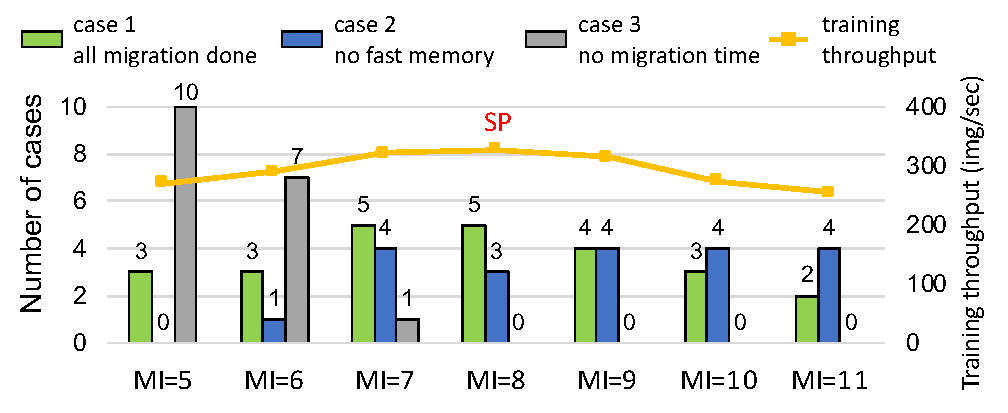
\includegraphics[width=0.5\textwidth]{figures/three_cases.pdf}
	\vspace{-25pt}
    \caption{\textcolor{check}{The occurrences of the three data migration cases in a training step of ResNet-32. ``MI'' stands for ``migration interval''. "SP" stands for sweet spot (the optimal migration interval). 
    }}
    \vspace{-10pt}
    \label{fig:migration_interval_three_cases}
\end{figure}
%\end{comment}
\begin{comment}
\begin{figure}
   \centering
\resizebox{0.48\textwidth}{0.3\textwidth}{
\begin{tikzpicture}
\pgfplotsset{
   width=0.5\textwidth,
   height=0.2\textheight,
  %% grid=major,
 %  major grid style={dotted},
   symbolic x coords={MI=5,MI=6,MI=7,MI=8,MI=9,MI=10,MI=11},
   enlarge y limits={upper,value=0.05},
   legend style={
      fill,
      at={(0.50,-0.4)},
      legend columns=4,
      legend cell align=left,
      anchor=north
      },
   }
\begin{axis}[
   xtick pos=left,
   axis y line*=left,
   ybar,
  % ymajorgrids,
   bar width=0.15cm,
  % ymin=0, ymax=1,
  % ytick={0, 0.25, 0.5, 0.75, 1},
 %  yticklabels={0, 25\%, 50\%, 75\%, 100\%},
   ylabel style={align=center},
   ylabel={Percentage of each case},
   xtick=data,
   xticklabel style={
      inner sep=0pt,
      anchor=north east,
      rotate=60
      }
   ]
   \addplot[ybar,ybar legend,fill=RYB1] coordinates {
      (MI=5,3) (MI=6,3) (MI=7,5)
      (MI=8,5) (MI=9,4) (MI=10,3)
      (MI=11,0.2) 
      };\label{AAA}   
   \addplot[ybar,ybar legend,fill=RYB2] coordinates {
     (MI=5,0) (MI=6,1) (MI=7,4)
      (MI=8,3) (MI=9,4) (MI=10,4)
      (MI=11,4) 
      };\label{BBB}     
   \addplot[ybar,ybar legend,fill=RYB3] coordinates {
       (MI=5,10) (MI=6,7) (MI=7,1)
      (MI=8,8) (MI=9,8) (MI=10,7)
      (MI=11,6) 
      };\label{CCC} 
\end{axis}
\begin{axis}[
   axis y line*=right,
   xticklabels={},
  ymin=0, ymax=400,
   ytick={0, 100, 200, 300, 400},
   ylabel={Training throughput\\ (img/sec)}%, nodes near coords,
    %nodes near coords %align={vertical}
   ]
   \addlegendimage{RYB1,/pgfplots/refstyle=AAA}
   \addlegendentry{Case 1}
   \addlegendimage{RYB2,/pgfplots/refstyle=BBB}
   \addlegendentry{Case 2}
      \addlegendimage{RYB3,/pgfplots/refstyle=CCC}
   \addlegendentry{Case 3}
   \addplot[very thick,draw=red,mark=square] plot coordinates {
      (MI=5,270.4) (MI=6,290.1) (MI=7,326.9)
      (MI=8,321.7) (MI=9,314.8) (MI=10,273.4)
      (MI=11,255.6) 
      };
   \addlegendentry{Training throughput}
   \end{axis}
\end{tikzpicture}
}
    \caption{How often the three data migration cases happen with different migration intervals. We use Resnet-32.}
    \label{fig:migration_interval_three_cases}
\end{figure}
\end{comment}

To avoid Case 2, long-lived tensors are immediately moved out of fast memory in the middle of $A$, once the remaining operations in $A$ do not need them. This saves space of fast memory. However, avoiding Case 3 is difficult, because it is created by the limited memory bandwidth and/or latency. 
In Case 3, we can either continue migrating data and let $B$ wait for the completion of data migration, or leave data in slow memory. The continuation of data migration exposes data migration into the critical path, but the execution of $B$ use data in fast memory; On the contrary, leaving data in slow memory uses the data in slow memory but avoids data migration overhead. This is a classic trade-off between data locality and data movement. To determine which method leads to the best performance, we use a test-and-trial algorithm.

In particular, whenever Case 3 happens at the end of an interval, we use one training step to try the continuation of data migration, and use another training step to try no-data-migration. We measure the performance of the two methods and use the best method in the remaining training steps. Note that in order to compare the performance of the two training steps, we must ensure that data placement in the two training steps is the same when Case 3 happens. The same data placement can be easily guaranteed, given the repetitive execution pattern in DNN training. 

The above algorithm does not cause large overhead, because Case 3 does not happen often and hence does not need a large amount of training steps for test and trial. The number of training steps used for test and trial is usually \textcolor{check}{less than 5}  (see Table~\ref{tab:models}). 
%two times of the number of migration intervals

%In practice, we find that \textcolor{red}{xxx} training steps are enough for DNN models in our evaluation. 
\vspace{-10pt}
\subsection{Discussions}
\label{sec:discussion}

\textbf{The lower bound of fast memory size.} Although fast memory can be smaller with \name, there is a lower bound of fast memory size to avoid big performance loss. This lower bound is the peak memory consumption of short-lived data objects \textcolor{check}{among all migration intervals} plus the largest long-lived data object. Smaller than this bound, the runtime system has to either frequently migrate short-lived data objects or has no space to accommodate long-lived data objects, which causes performance loss larger than 10\%. 


\textbf{Handling dynamic graphs.}
Some machine learning frameworks, such as PyTorch and TensorFlow 2.0, support dynamic graphs. \textcolor{check}{Depending on the size of input within a batch, these frameworks generate a different dataflow graph with a right shape to accommodate the batch}.
%%%With dynamic graphs, batches are not identical. 
Hence, there could be multiple graphs. 

To handle dynamic graphs, the existing solution pads zero at the end of input~\cite{google_tensorflow_bucketing}, such that batches have the same structure. This transforms a dynamic graph into a static one, but at the cost of larger memory footprint and unnecessary computation. We use a solution similar to the one in~\cite{DBLP:conf/asplos/SivathanuCSZ19} that uses bucketed profiling. In particular, \name bucketizes the input sizes into a small  \textcolor{dong2}{number} of buckets (at most 10 in \name
), and each bucket has a similar graph. \name profiles each bucket to collect memory access information and decide data migration. 


\textbf{Handling control dependencies.}
A static graph can have control flow. Depending on the value of input in a batch, the graph can have different dataflow, causing different memory access patterns. \name handles this case by tracking dataflow. Whenever a new dataflow is encountered, \name triggers profiling and makes the decision of data migration again. 

\textcolor{check}{\textbf{Support of dynamic migration interval.} In \name, all migration intervals use the same value (i.e., the number of layers). An alternative approach is to use different values for different intervals. Using such a dynamic migration interval is helpful to avoid Cases 2 and 3. However, this method brings few performance benefit in practice, because Cases 2 and 3 do not happen often (shown in Table~\ref{tab:models}). Also, determining appropriate dynamic migration intervals has to explore a large search space of migration intervals, which can cause larger runtime overhead.}